\documentclass{beamer}

\usepackage{graphicx}
\usepackage{listings}

\title{6.111 Final Project: Radio Society Defense Network}
\author{Oliver Trevor}
\institute{MIT}
\date{October 31, 2022}

\begin{document}
    \frame{\titlepage}

    \begin{frame}
        \frametitle{Problem Overview}
        \begin{itemize}
            \item Trolls and interfering transmissions are a significant problem for amateur radio repeaters

            \item Current publicly-available RF fingerprinting solutions are retroactive, so they cannot prevent interference while it's happening

            \item Fingerprinting the keyup characteristics caused by instabilities in the PLL of an FM transceiver lets us uniquely identify people

            \item Doing this on an FPGA makes real-time lockout of unwanted users (without delaying normal users' transmissions) possible
        \end{itemize}
    \end{frame}

    \begin{frame}
        \frametitle{Block Diagram}

        \centerline{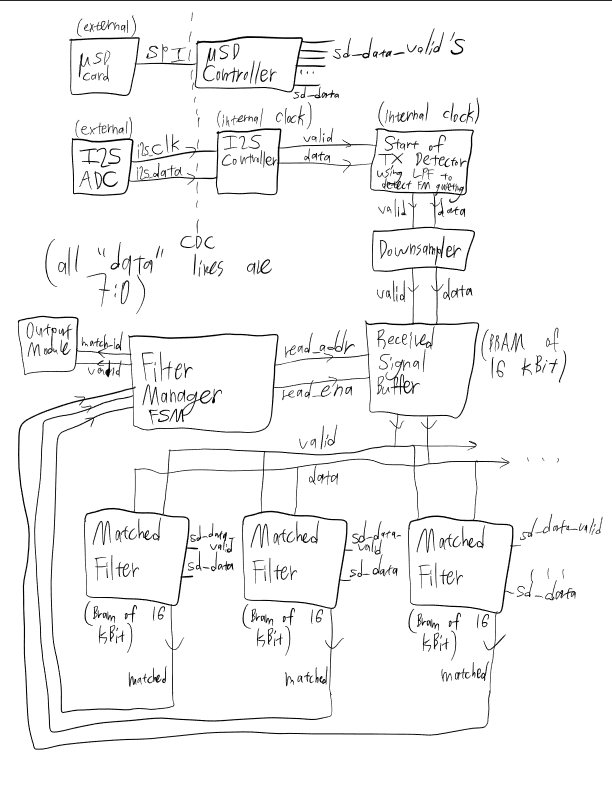
\includegraphics[width=7cm]{Block_Diagram_Drawing.png}}
    \end{frame}

    \begin{frame}
        \frametitle{Changes -- Start of Transmission Filtering}

        \begin{columns}
            \begin{column}{.5\textwidth}
                \centerline{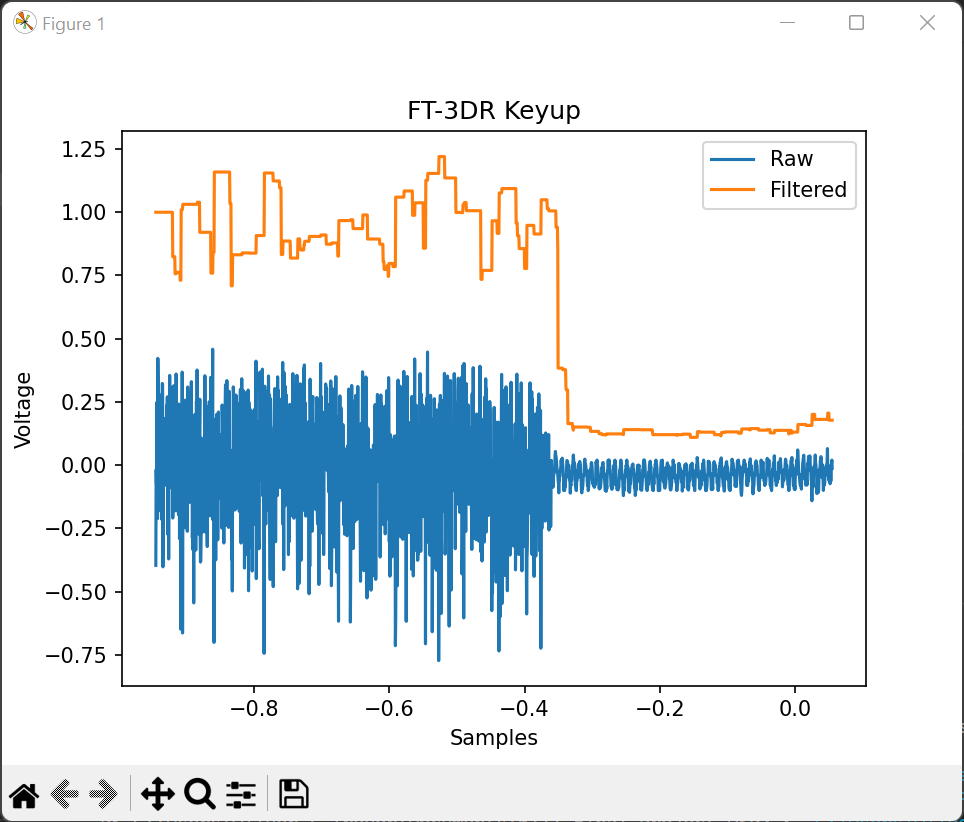
\includegraphics[width=6cm]{ft3dr_keyup.png}}
            \end{column}
            \begin{column}{.5\textwidth}
                \begin{itemize}
                    \item<only@1> Developed working algorithm for detecting start of transmission cheaply on FPGA and tested it with a DSO and Python

                    \item<only@1> Track the difference between the \emph{maximum} and the \emph{minimum} of the previous 50 samples

                    \item<only@2> Detect when that difference drops sharply -- gets us an effect similar to an LPF or an envelope detector but without the complexity

                    \item<only@2> Audio samples are spaced out enough that we have time in between to search through a buffer of samples to find minimum and maximum
                \end{itemize}
            \end{column}
        \end{columns}
    \end{frame}

    \begin{frame}
        \frametitle{Changes -- Matched Filter Design}

        \begin{itemize}
            \item<only@1> Decided to start out with time-domain correlators only (not frequency-domain)

            \item<only@1> Frequency-domain correlators each require their own iFFT module to be useful

            \item<only@1> Attempted to develop a ``shortcut" method to identify match/no match from convolved FFT without doing iFFT -- not going to work very well

            \item<only@2> Time-domain correlators will use multiply-accumulators from DSP slices

            \item<only@2> On each clock cycle, read \lstinline{SAMPLES_PER_CLOCK} samples from receive buffer and multiply them by the corresponding values read from internal fingerprint buffer

            \item<only@2> A second stage in the pipeline will ``accumulate" (sum) the results of the multiplications

            \item<only@2> Once the entire dot product has been computed, phase shift by \lstinline{CONVOLUTION_RESOLUTION} samples, reset the accumulator, and go back to multiply-accumulating

            \item<only@2> Use a register storing the maximum accumulator value so far -- this value will be the final output of the filter
        \end{itemize}
    \end{frame}

    \begin{frame}
        \frametitle{Changes -- Matched Filter Optimization Parameters}

        \begin{itemize}
            \item Can change the number of multiplies performed in one clock cycle by a filter module to trade off area and throughput -- since receive is buffered, we can pull in as many samples as we want

            \item Can change the amount that we phase shift the fingerprint and the receive buffer between dot products to take a ``sparser" convolution to tradeoff accuracy and throughput

            \item Can change the total number of filter modules

            \item Can change the overall clock speed the filters run at

            \item Can downsample bit depth and sample rate to tradeoff accuracy and total processing time
        \end{itemize}
    \end{frame}

    \begin{frame}
        \frametitle{Changes -- Filter Manager FSM Details}

        \begin{itemize}
            \item Starts by loading all available fingerprints from uSD controller into BRAMs of filters

            \item Lets filters run, then decides which one got the best positive match (or that none did)

            \item Makes decision based on match strength whether we go to next ``bank" of fingerprints -- if so, swap in a different set of fingerprints into the BRAMs and run the filters on those
        \end{itemize}
    \end{frame}

    \begin{frame}
        \frametitle{Evaluating Design Efficacy}

        \begin{itemize}
            \item Overall latency from start of transmission to block/no block signal output must be less than 0.2-0.3 seconds

            \item The entire available time from end of keyup to start of voice transmission (minus repeater keyup time) should be used to fit as many computations as possible

            \item All available BRAM should be used

            \item Design should be able to run at 100 MHz minimum, 150 or 200 MHz would be nice

            \item Design throughput will be measured as the total number of matched filter operations we can perform in a given time
        \end{itemize}
    \end{frame}

    \begin{frame}
        \frametitle{Timeline}

        \begin{itemize}
            \item Week 1 -- Working matched filter design that correctly performs a correlation on signals loaded from ROMs
            \item Week 2 -- Working data reading from I2S (or possibly not I2S) ADC into BRAM buffer
            \item Week 3 -- Working fingerprint loading from microSD card
            \item Week 4 -- Working management FSM (this is the minimum viable product point)
            \item Week 5 -- Optimization
            \item Week 6 -- Optimization
            \item Week 7 -- Final report writing
        \end{itemize}
    \end{frame}

    \begin{frame}
        \frametitle{Checkoffs}

        \begin{itemize}
            \item Commitment -- working matched filter module that produces a correlation value matching Python's result for the same data, working uSD module that loads data from BRAMs, working FSM that runs at least 1 comparison on each matched filter module, working ADC reading, working output to repeater controller
            \item Goal -- (same as commitment) PLUS working FSM that ``re-uses" matched filter modules with multiple fingerprints so that we can fill up all available computation time even if we run out of area to create extra filters PLUS communicating with a computer for logging identifications
            \item Stretch goal -- (same as goal) PLUS some kind of system, possibly in conjunction with the computer, for recording transmissions so that you can go back and retroactively attach names to people to be able to identify them in future PLUS management of fingerprint library without putting SD card in a computer (i. e. some kind of management protocol over Ethernet/RS-232)
        \end{itemize}
    \end{frame}
\end{document}
